\documentclass[13pt,a4paper]{report}
\usepackage[utf8]{inputenc}
\usepackage[portuguese]{babel}
\usepackage[T1]{fontenc}
\usepackage[fleqn]{amsmath}
\usepackage{amsfonts}
\usepackage{amssymb}
\usepackage{graphicx}
\usepackage{fancyhdr}
\usepackage{indentfirst}
\usepackage{listings}
\usepackage{color}
\usepackage{hyperref}

\definecolor{mygreen}{rgb}{0,0.6,0}
\definecolor{mygray}{rgb}{0.5,0.5,0.5}
\definecolor{mymauve}{rgb}{0.58,0,0.82}

\pagestyle{fancy}

\lstset{language=Java}   

\lstset{ %
  backgroundcolor=\color{white},   % choose the background color; you must add \usepackage{color} or \usepackage{xcolor}
%  basicstyle=\footnotesize,        % the size of the fonts that are used for the code
  basicstyle=\ttfamily\scriptsize,
  breakatwhitespace=false,         % sets if automatic breaks should only happen at whitespace
  breaklines=true,                 % sets automatic line breaking
  captionpos=b,                    % sets the caption-position to bottom
  commentstyle=\color{mygreen},    % comment style
  deletekeywords={...},            % if you want to delete keywords from the given language
  escapeinside={\%*}{*)},          % if you want to add LaTeX within your code
  extendedchars=true,              % lets you use non-ASCII characters; for 8-bits encodings only, does not work with UTF-8
  frame=single,                    % adds a frame around the code
  keepspaces=true,                 % keeps spaces in text, useful for keeping indentation of code (possibly needs columns=flexible)
  keywordstyle=\color{blue},       % keyword style
  language=Octave,                 % the language of the code
  morekeywords={*,...},            % if you want to add more keywords to the set
  numbers=left,                    % where to put the line-numbers; possible values are (none, left, right)
  numbersep=5pt,                   % how far the line-numbers are from the code
  numberstyle=\tiny\color{mygray}, % the style that is used for the line-numbers
  rulecolor=\color{black},         % if not set, the frame-color may be changed on line-breaks within not-black text (e.g. comments (green here))
  showspaces=false,                % show spaces everywhere adding particular underscores; it overrides 'showstringspaces'
  showstringspaces=false,          % underline spaces within strings only
  showtabs=false,                  % show tabs within strings adding particular underscores
  stepnumber=2,                    % the step between two line-numbers. If it's 1, each line will be numbered
  stringstyle=\color{mymauve},     % string literal style
  tabsize=2,                       % sets default tabsize to 2 spaces
  title=\lstname                   % show the filename of files included with \lstinputlisting; also try caption instead of title
}


\lhead{Pêndulo Duplo e Pêndulo Impulsionado}
\rhead{Pág. \thepage}
\renewcommand{\footrulewidth}{0.4pt}% default is 0pt
\cfoot{Jelther Oliveira Gonçalves}



%\renewcommand*{\familydefault}{\sfdefault}



\begin{document}

	\title{Pêndulo Duplo e Pêndulo Impulsionado em HTML5 e JavaScript}
	\author{Jelther Gonçalves\\		
	 \\
 	 Instituto de Matemática, Estatística e Computação Científica\\
	 Universidade Estadual de Campinas\\
	 \\
	 Curso de Matemática Aplicada e Computacional\\
	 \\
	 E-mail: \texttt{\href{mailto:jetolgon@gmail.com}{jetolgon@gmail.com}}}
	\date{\today}	
	\maketitle
	
	\begin{abstract}
	
Este trabalho visa fornecer uma simulação computacional do pêndulo duplo e do pêndulo impulsionado em seu pivô.

As simulações são construídas utilizando a tecnologia HTML5 e Javascript, facilitando sua visualização em diferentes dispositivos e plataformas sem a necessidade de componentes extras.
	\end{abstract}
	
	\tableofcontents
	\clearpage

	\chapter{Pêndulo Impulsionado}	
	\section{Dedução das equações}
	
	Um pêndulo é um sistema composto por uma massa acoplada a um pivô que permite sua movimentação livremente.
	
No pêndulo impulsionado, partiremos do princípio que o pivô irá se mover de forma oscilatória verticalmente ou horizontalmente.
Vamos iniciar com o pêndulo impulsionado verticalmente:

\begin{center}
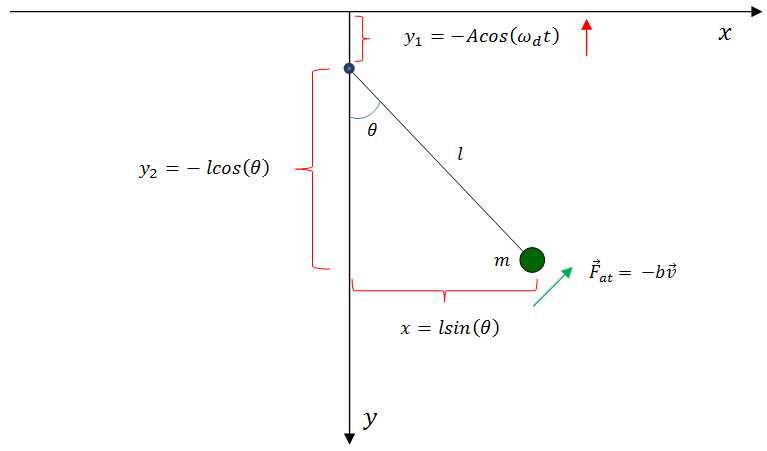
\includegraphics[scale=0.6]{figuras/esquemapenduloimpulsionado.png}
\end{center}
\clearpage

No esquema acima utilizamos x e y como coordenadas generalizadas para o pêndulo.Como podemos ver, o pivô se move verticalmente em função de um cosseno e uma amplitude.
\\

Para obtermos a equação do movimento, devemos utilizar os conceitos de mecânica lagrangiana. Ou seja, devemos ter L = T - U, onde T é a soma das energias cinéticas e U a soma das energias potenciais do sistema.
\\
Portanto, T fica:
\begin{center}
$
 T = \frac{1}{2}m(\dot{x}^{2} + \dot{y}^{2})
$
\end{center}

Onde o ponto denota a derivada temporal. Os valores x e y serão as somas dos encontrados no esquema acima, então:

\begin{center}
$
	\dot{x} = l\dot{\theta}\cos\theta	
$
\\[2mm]
$
	\dot{y} = - l\dot{\theta}\sin\theta -A\omega_{d}\sin(\omega_{d} t)
$
\\[2mm]
$
	\dot{x}^{2} + \dot{y}^{2} = l^{2}\dot{\theta}^{2}\cos^{2}\theta	
	+ l^{2}\dot{\theta}^{2}\sin^{2}\theta	
	+ A^{2}\omega_{d}^{2}\sin^{2}(\omega_{d} t)
	+ 2l\dot{\theta}A\omega_{d}\sin(\omega_{d} t)
$
\end{center}

Simplificando esta última, obteremos T:
\begin{center}
$
	T = \dfrac{m}{2}
	( l^{2}\dot{\theta}^{2} 
	  + A^{2}\omega_{d}^{2}\sin^{2}(\omega_{d} t)
	  + 2l\dot{\theta}A\omega_{d}\sin(\omega_{d} t)
	)
$
\end{center}

O próximo passo é encontrar a energia potencial U:
\begin{center}
$
 U = -mgy = 	-mg(l\cos\theta + A\cos(\omega_{d} t))
$
\end{center}

Portanto, a Lagrangiana será:
\begin{center}
$
 L = \dfrac{m}{2}
	( l^{2}\dot{\theta}^{2} 
	  + A^{2}\omega_{d}^{2}\sin^{2}(\omega_{d} t)
	  + 2l\dot{\theta}A\omega_{d}\sin(\omega_{d} t)
 ) + mg(l\cos\theta + A\cos(\omega_{d} t))
$
\end{center}

Vamos notar que existe uma força de atrito proporcional a velocidade da esfera. Esta força pode ser generalizada da seguinte forma:
\\
\begin{center}
$
 Q_{\theta} = F_{atx}\dfrac{\partial x}{\partial \theta}
 			  + F_{aty}\dfrac{\partial y}{\partial \theta}
$
\end{center}
\clearpage


Portanto, vamos encontrar  $ F_{atx} $  e $ F_{aty} $:
\begin{center}
$
F_{atx} = -b\dot{x} = -bl\cos\theta\dot{\theta}
$
\\[2mm]
$
F_{aty} = -b\dot{y} = -bl\sin\theta\dot{\theta} + Ab\omega_{d}\sin(\omega_{d}t)
$
\\[2mm]
$
\dfrac{\partial x}{\partial \theta} = l\cos\theta
$
, 
$
\dfrac{\partial y}{\partial \theta} = l\sin\theta
$
\end{center}

Então, $Q_{\theta}$ fica:

\begin{center}
$
Q_{\theta} = 
-b\dot{\theta}l^{2}\cos^{2}\theta
-b\dot{\theta}l^{2}\sin^{2}\theta
+Abl\omega_{d}\sin\theta\sin(\omega_{d} t)
$
\\[2mm]
$
Q_{\theta} = 
-b\dot{\theta}l^{2}
+Abl\omega_{d}\sin\theta\sin(\omega_{d} t)
$
\end{center}

Finalmente, podemos determinar a equação de $ \dot{\theta} $
a partir da definição da Lagrangiana:
\begin{center}
$
\dfrac{d}{dt} \left(\dfrac{\partial L}{\partial \dot{\theta}}\right)
- \dfrac{\partial L}{\partial \theta} = Q_{\theta}
$
\\[2mm]
$
\dfrac{\partial L}{\partial \dot{\theta}} = 
ml^{2}\dot{\theta} + mlA\omega_{d}\sin\theta\sin(\omega_{d} t)
$
\\[2mm]
$
\dfrac{d}{dt} \left(\dfrac{\partial L}{\partial \dot{\theta}}\right) = 
ml^{2}\ddot{\theta} 
+ mlA\omega_{d}\dot{\theta}\cos\theta\sin(\omega_{d} t)
+ mlA\omega_{d}^{2}\sin\theta\cos(\omega_{d} t)
$
\\[2mm]
$
\dfrac{\partial L}{\partial \theta} = 
mlA\omega_{d}\dot{\theta}\cos\theta\sin(\omega_{d} t)
-mgl\sin\theta
$
\end{center}

Chegamos então em:
\begin{center}
$
\ddot{\theta} = 
-\sin\theta
\left[\dfrac{A\omega_{d}^{2} \cos(\omega_{d} t) + g }{l}\right]
+ \dfrac{Q_{\theta}}{ml^{2}}
$
\end{center}

Esta equação é a que descreve o movimento da massa ao redor do pivô.
\clearpage

	\section{Adequando para  o método de Runge-Kutta de 4ª Ordem}
	
	Claramente, a equação do movimento não possui uma solução analítica.Para resolver esta equação, devemos utilizar um método numérico.
	
	O método utilizado para o desenvolvimento do applet é o de Runge-Kutta de 4ª Ordem.No apêndice A descrevemos como o método funciona para casos gerais.

Realizando uma mudança de variáveis ficamos com o seguinte sistema de equações diferenciais de primeira ordem:
\\[2mm]
$ \left\{
\begin{array}{ll}

 	\dot{\theta}  = \omega \\
	 	\dot{\omega}  = -\sin\theta\ 	 	
	 	\left[\dfrac{A\omega_{d}^{2} \cos(\omega_{d} t) + g }{l}\right]
	 	+ \dfrac{1}{ml^{2}} 	\left( -bl^{2}\omega + Abl\omega_{d}\sin\theta\sin(\omega_{d}t)	\right) \\
	 t = 1

\end{array}
\right.
$
\\[2mm]

Ou seja,
\\[2mm]
$
\left\{
\begin{array}{ll}
 	\dot{\theta}  = f(t,\theta,\omega) \\
 	\dot{\omega}  = g(t,\theta,\omega) \\ 	
	 t = l(t,\theta,\omega) \\
\end{array}
\right.
$
\\[2mm]

Onde $f$,$g$ e $k$ são as funções acima representadas.Utilizaremos parâmetros extras ao escrever as 
funções (como $t$ para função $f$) para que não haja confusão na construção do método numérico.
\clearpage
Portanto, a implementação em Javascript do método numérico é:
\begin{lstlisting}
function f(tempo,theta,vel_angular) {                      
 temp = -(gravidade + Amp*omegad*omegad*Math.cos(omegad*tempo))*Math.sin(theta);
 temp = temp/(comprimento_pendulo1);
 temp = temp -((b_damping/massa1)*vel_angular) + (Amp*b_damping*omegad*Math.sin(theta)*Math.sin(omegad*tempo))/(massa1*comprimento_pendulo1);     
 return temp;    
}

function g(tempo,theta,vel_angular) {   
  return vel_angular;
}

function k(tempo,theta,vel_angular) {
 return 1;
}
           
function rungeKuttaPendulo(timediff) {    
 var h = timediff/1000;
 var a = [];
 var b = [];
 var c = [];
 var d = [];

 a[1] = g(tempo_n, theta_n_1 , vel_angular_n_1);
 a[2] = f(tempo_n, theta_n_1 , vel_angular_n_1);
 a[3] = k(tempo_n, theta_n_1 , vel_angular_n_1);

 b[1] = g(tempo_n + (h/2)*a[3] , theta_n_1 + (h/2)*a[1] , vel_angular_n_1 + (h/2)*a[2] );
 b[2] = f(tempo_n + (h/2)*a[3] , theta_n_1 + (h/2)*a[1] , vel_angular_n_1 + (h/2)*a[2] );
 b[3] = k(tempo_n + (h/2)*a[3] , theta_n_1 + (h/2)*a[1] , vel_angular_n_1 + (h/2)*a[2] );
        
 c[1] = g(tempo_n + (h/2)*b[3] , theta_n_1 + (h/2)*b[1] , vel_angular_n_1 + (h/2)*b[2] );
 c[2] = f(tempo_n + (h/2)*b[3] , theta_n_1 + (h/2)*b[1] , vel_angular_n_1 + (h/2)*b[2] );
 c[3] = k(tempo_n + (h/2)*b[3] , theta_n_1 + (h/2)*b[1] , vel_angular_n_1 + (h/2)*b[2] );

 d[1] = g(tempo_n + h*c[3] , theta_n_1 + h*c[1] , vel_angular_n_1 + h*c[2] );
 d[2] = f(tempo_n + h*c[3] , theta_n_1 + h*c[1] , vel_angular_n_1 + h*c[2] );
 d[3] = k(tempo_n + h*c[3] , theta_n_1 + h*c[1] , vel_angular_n_1 + h*c[2] );
                
 theta_n_1 = theta_n_1 + (h/6)*(a[1] + 2*b[1] + 2*c[1] + d[1]); 
 vel_angular_n_1 = vel_angular_n_1 + (h/6)*(a[2] + 2*b[2] + 2*c[2] + d[2]);     
 tempo_n = tempo_n + (h/6)*(a[3] + 2*b[3] + 2*c[3] + d[3]); 
    
 delete a;delete b;delete c;delete d;
}
\end{lstlisting}
\clearpage

\section{Mudança do ponto estável}
Podemos perceber (experimentalmente) que o pêndulo muda seu comportamento quando escolhemos ângulos iniciais diferentes.

A mudança principal é o seu ponto estável : quando colocado a partir de um ângulo o mesmo fica estável acima do eixo Y.
\\[1mm]

Vamos tomar como exemplo os valores :
\begin{center}
Massa = $ 13 \ Kg $
\\[1mm]Coef. Amortecimento = $ 1 \ Kg/s $
\\[1mm]Vel. Angular Inicial = $ 0 \ rad/s $
\\[1mm]Frequência de Vibração = $ 5 \ Hz $
\\[1mm]Amplitude do Impulso = $ 0.3 \ m $
\\[1mm]Comprimento do Pêndulo = $ 3 \ m $
\\[1mm]Gravidade = $ 9.8 \ m/s^{2} $
\end{center}
Com estes valores, vemos que o pêndulo se mantem estável 
na vertical a partir de $ \pm136^{\underline{o}} = \pm2.374 \ rad$ em relação ao eixo Y.

\begin{center}
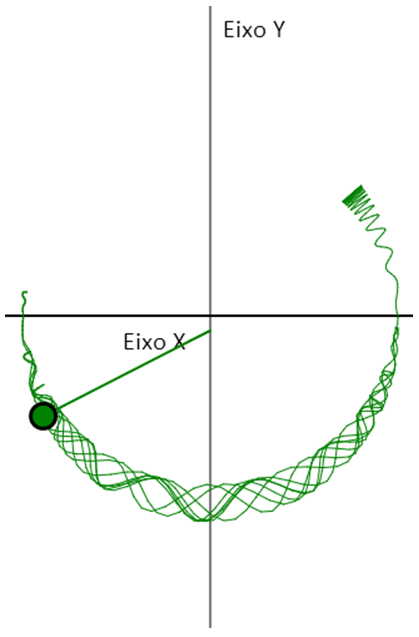
\includegraphics[scale=0.5]{figuras/tracopenduloimpulsionado135.png}
\\
\textit{Figura 1: Traço do pêndulo após $14 s$ de movimento em um ângulo inicial
de $135^{\underline{o}}$ }
\end{center}
\clearpage


\begin{center}
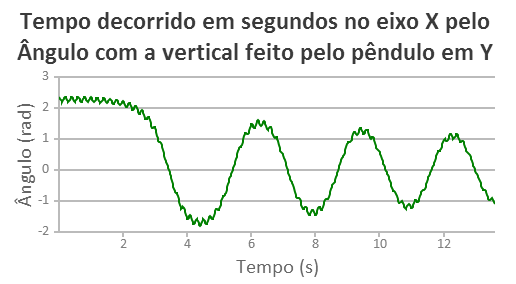
\includegraphics[scale=0.9]{figuras/graficopenduloimpulsionado135.png}
\\
\textit{Figura 2: Gráfico do pêndulo após $14 s$ de movimento em um ângulo inicial
de $135^{\underline{o}}$ }
\end{center}

\begin{center}
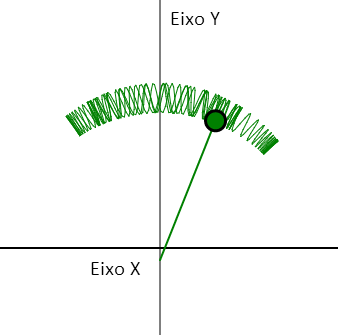
\includegraphics[scale=0.9]{figuras/tracopenduloimpulsionado136.png}
\\
\textit{Figura 3: Traço do pêndulo após $14 s$ de movimento em um ângulo inicial
de $136^{\underline{o}}$ }
\end{center}
\clearpage


\begin{center}
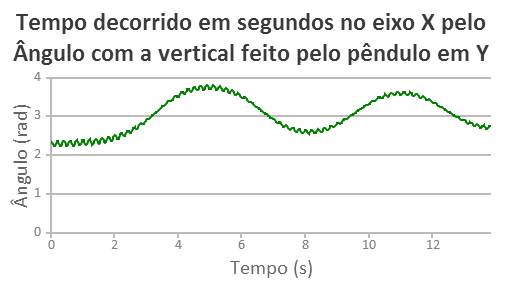
\includegraphics[scale=0.9]{figuras/graficopenduloimpulsionado136.png}
\\
\textit{Figura 4: Gráfico do pêndulo após $14 s$ de movimento em um ângulo inicial
de $136^{\underline{o}}$ }
\end{center}
\clearpage

\section{Movimento caótico do pêndulo impulsionado}

Este pêndulo apresenta comportamento caótico dependendo dos parâmetros iniciais que utilizamos, isto é, é impossível determinar seu movimento.

Vamos tomar como exemplo os seguintes parâmetros iniciais e comparar os traços e gráficos gerados:

\begin{center}
Massa = $ 13 \ Kg $
\\[1mm]Coef. Amortecimento = $ 0 \ Kg/s $
\\[1mm]Vel. Angular Inicial = $ 0 \ rad/s $
\\[1mm]Frequência de Vibração = $ 0.79\pi \ rad/s = 0.39 \ Hz $
\\[1mm]Amplitude do Impulso = $ 0.7 \ m $
\\[1mm]Comprimento do Pêndulo = $ 3 \ m $
\\[1mm]Gravidade = $ 9.8 \ m/s^{2} $
\end{center}

Comparando os traços, gráficos e diagramas:


\begin{center}
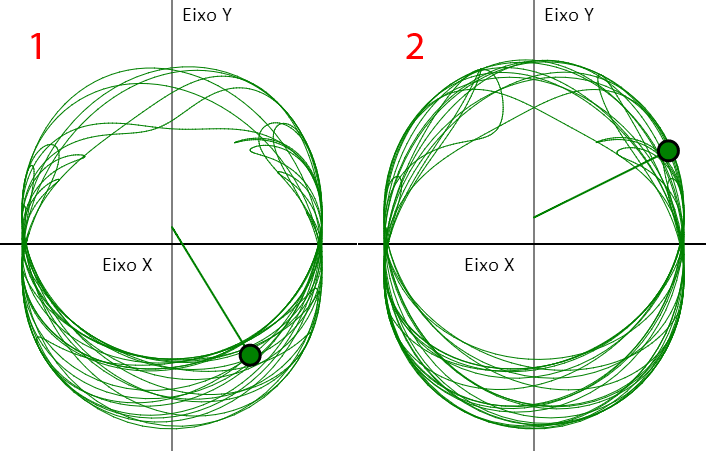
\includegraphics[scale=0.5]{figuras/figura5.png}
\\
\textit{Figura 5: Traço dos pêndulos após $60 s$ de movimento em um ângulo inicial de $-108^{\underline{o}}$ }
\end{center}
\clearpage

\begin{center}
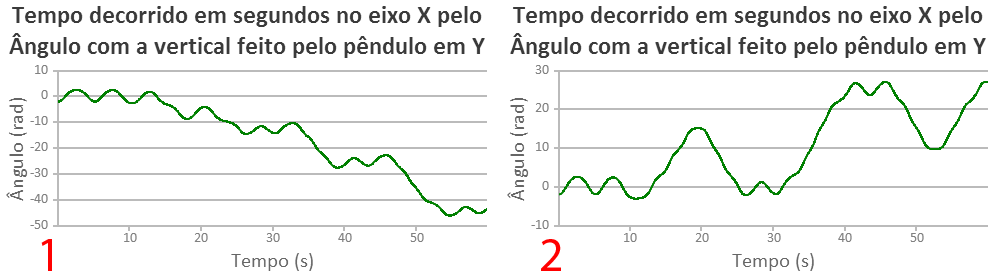
\includegraphics[scale=0.5]{figuras/figura6.png}
\\
\textit{Figura 6: Gráfico dos pêndulos após $60 s$ de movimento em um ângulo inicial de $-108^{\underline{o}}$ }
\end{center}

\begin{center}
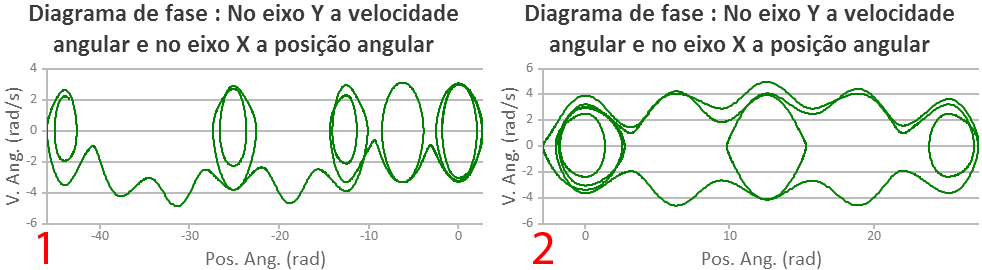
\includegraphics[scale=0.5]{figuras/figura7.png}
\\
\textit{Figura 7: Diagramas de fase  após $60 s$ de movimento em um ângulo inicial de $-108^{\underline{o}}$ }
\end{center}

Através disso, podemos confirmar o movimento caótico que pode ser causado a partir de mesmos valores iniciais.
\clearpage

\chapter{O Pêndulo Duplo}	
\section{Dedução das equações}

O pêndulo duplo consiste em um pêndulo acoplado a outro pêndulo através de sua massa.Em nosso caso, ilustraremos estes pêndulos como sendo simples.

Para certas condições, este sistema apresenta um comportamento caótico também. Vamos iniciar então com a dedução das equações do movimento deste sistema através da mecânica Lagrangiana.

\begin{center}
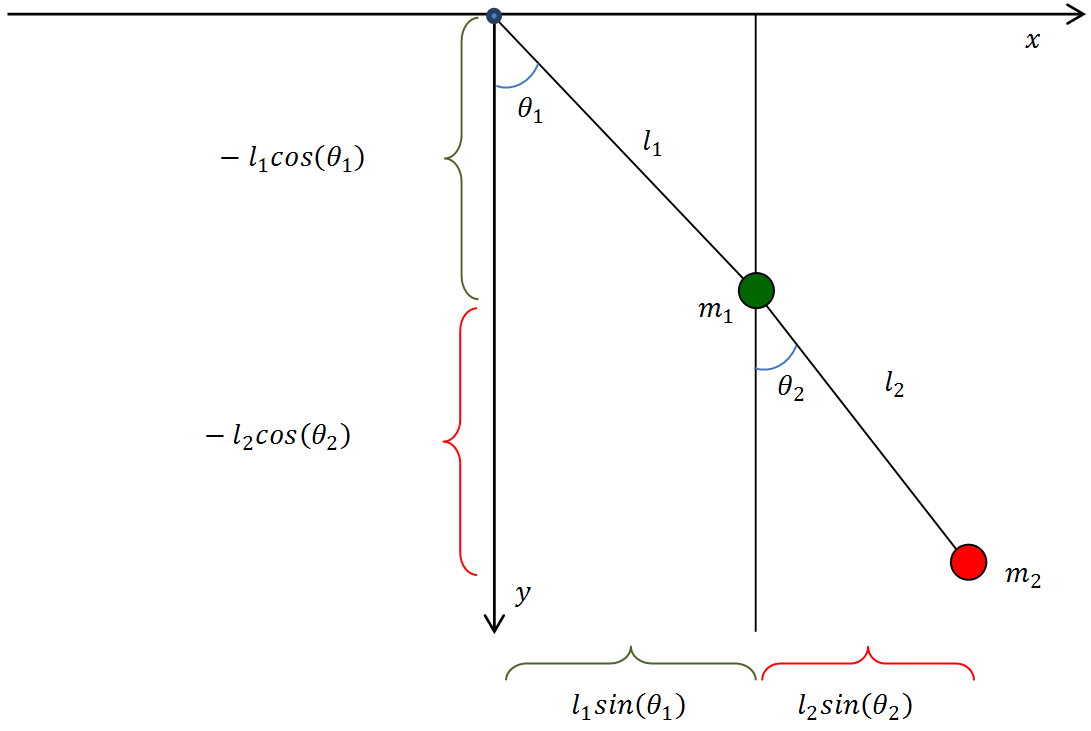
\includegraphics[scale=0.4]{figuras/esquemapenduloduplo.png}
\end{center}
\clearpage

Portanto, vamos calcular as energias envolvidas:

Massa 1:
\begin{center}
$
\dot{x_{1}} = l_{1}\dot{\theta_{1}}\cos\theta_{1}
$
e
$
\dot{y_{1}} = l_{1}\dot{\theta_{1}}\sin\theta_{1}
$
\\[2mm]
$
\dot{x}_{1}^{2} + \dot{y}_{1}^{2} = l_{1}^{2}\dot{\theta}_{1}^{2}
$
\end{center}

Massa 2:

\begin{center}
$
\dot{x_{2}} = l_{1}\dot{\theta_{1}}\cos\theta_{1} 
			+ l_{2}\dot{\theta_{2}}\cos\theta_{2}
$
\\[2mm]
$
\dot{y_{2}} = l_{1}\dot{\theta_{1}}\sin\theta_{1}
			+ l_{2}\dot{\theta_{2}}\sin\theta_{2}
$
\\[2mm]
$
\dot{x}_{2}^{2} + \dot{y}_{2}^{2} = l_{1}^{2}\dot{\theta}_{1}^{2}
+ 2l_{1}l_{2}\dot{\theta}_{1}\dot{\theta}_{2}\cos(\theta_{1} - \theta_{2})
+ l_{2}^{2}\dot{\theta}_{2}^{2}
$
\end{center}
Então, T fica:
\begin{center}
$
T  = \dfrac{m_{1}}{2}(\dot{x}_{1}^{2} + \dot{y}_{1}^{2}) 
	+ \dfrac{m_{2}}{2}(\dot{x}_{2}^{2} + \dot{y}_{2}^{2}) 
$
\\[2mm]
$
T  = \dfrac{m_{1}}{2}( l_{1}^{2}\dot{\theta}_{1}^{2} ) 
	+ \dfrac{m_{2}}{2}( l_{1}^{2}\dot{\theta}_{1}^{2}
+ 2l_{1}l_{2}\dot{\theta}_{1}\dot{\theta}_{2}\cos(\theta_{1} - \theta_{2})
+ l_{2}^{2}\dot{\theta}_{2}^{2} ) 
$
\\[2mm]
$
T  = \dfrac{ (m_{1} + m_{2}) }{2}( l_{1}^{2}\dot{\theta}_{1}^{2} ) 
	+ m_{2}l_{1}l_{2}\dot{\theta}_{1}\dot{\theta}_{2}\cos(\theta_{1} - \theta_{2})		+ \dfrac{m_{2}}{2}( l_{2}^{2}\dot{\theta}_{2}^{2} ) 
$
\end{center}
A energia potencial U depende somente de y, então:

Massa 1:
\begin{center}
$
U = -m_{1}gl_{1}\cos\theta_{1}
$
\end{center}

Massa 2:
\begin{center}
$
U = -m_{2}g ( l_{1}\cos\theta_{1} + l_{2}\cos\theta_{2} )
$
\end{center}

Então a energia U total será:
\begin{center}
$
U = -m_{1}gl_{1}\cos\theta_{1} -m_{2}g ( l_{1}\cos\theta_{1} + l_{2}\cos\theta_{2} )
$
\\[2mm]
$
U = -(m_{1} + m_{2}) gl_{1}\cos\theta_{1} -m_{2}gl_{2}\cos\theta_{2}
$
\end{center}
A Lagrangiana será:
\begin{center}
$
L = T - U
$
\\[2mm]
$
L = \dfrac{(m_{1} + m_{2})}{2}l_{1}^{2}\dot{\theta}_{1}^{2} 
	+ \dfrac{m_{2}}{2}\left( l_{2}^{2}\dot{\theta}_{2}^{2} \right)
	+ m_{2}l_{1}l_{2}\dot{\theta}_{1}\dot{\theta}_{2}\cos\left(\theta_{1} - \theta_{2}\right)
	+ \left(m_{1} + m_{2}\right)gl_{1}\cos\theta_{1}
	+ m_{2}gl_{2}\cos\theta_{2}
$
\end{center}
\clearpage
Para obter a equação para $\theta_{1}$, devemos calcular os termos:
\begin{center}
$
\dfrac{\partial L}{\partial\dot{\theta}_{1}} =
\left(m_{1} + m_{2}\right)l_{1}^{2}\dot{\theta}_{2}
+ m_{2}l_{1}l_{2}\dot{\theta}_{2}\cos\left(\theta_{1} - \theta_{2}\right)
$
\\[2mm]
$
\dfrac{d}{dt}\left( \dfrac{\partial L}{\partial\dot{\theta}_{1}} \right) =
\left(m_{1} + m_{2}\right)l_{1}^{2}\ddot{\theta}_{1}
+ m_{2}l_{1}l_{2}\ddot{\theta}_{2}\cos\left(\theta_{1} - \theta_{2}\right)
+ m_{2}l_{1}l_{2}\dot{\theta}_{2}\sin\left(\theta_{1} - \theta_{2}\right)\left(\dot{\theta}_{1} - \dot{\theta}_{2} \right)
$
\\[2mm]
$
\dfrac{\partial L}{\partial\theta_{1}} = -l_{1}g\left(m_{1} + m_{2} \right)
-m_{2}l_{1}l_{2}\dot{\theta}_{1}\dot{\theta}_{2}\sin\left(\theta_{1} - \theta_{2}\right)
$
\end{center}
Então, ficamos com:
\begin{center}
$
\left(m_{1} + m_{2}\right)l_{1}^{2}\ddot{\theta}_{1}
+ m_{2}l_{1}l_{2}\ddot{\theta}_{2}\cos\left(\theta_{1} - \theta_{2}\right)
+m_{2}l_{1}l_{2}\dot{\theta}_{2}^{2}\sin\left(\theta_{1} - \theta_{2}\right)
+l_{1}g\left(m_{1} + m_{2}\right)\sin\left(\theta_{1}\right) = 0
$
\end{center}
Que simplificando por $l_{1}$, fica:
\begin{center}
$
\left(m_{1} + m_{2}\right)l_{1}\ddot{\theta}_{1}
+ m_{2}l_{2}\ddot{\theta}_{2}\cos\left(\theta_{1} - \theta_{2}\right)
+m_{2}l_{2}\dot{\theta}_{2}^{2}\sin\left(\theta_{1} - \theta_{2}\right)
+g\left(m_{1} + m_{2}\right)\sin\left(\theta_{1}\right) = 0
$
\end{center}
De forma análoga para $\theta_{2}$:
\begin{center}
$
\dfrac{\partial L}{\partial \dot{\theta}_{2}} =
m_{2}l_{2}^{2}\dot{\theta}_{2} +
m_{2}l_{1}l_{2}\dot{\theta}_{1}\cos\left(\theta_{1} - \theta_{2}\right)
$
\\[2mm]
$
\dfrac{d}{dt}\left(\dfrac{\partial L}{\partial\dot{\theta}_{2}}\right) = m_{2}l_{2}^{2}\ddot{\theta}_{2} + m_{2}l_{1}l_{2}\ddot{\theta}_{1}\cos\left(\theta_{1} - \theta_{2}\right) - m_{2}l_{1}l_{2}\dot{\theta}_{1}\sin\left(\theta_{1} -\theta_{2}\right)\left(\dot{\theta}_{1} - \dot{\theta}_{2} \right)
$
\\[2mm]
$
\dfrac{\partial L}{\partial \theta_{2}} =
m_{2}l_{1}l_{2}\dot{\theta}_{1}\dot{\theta}_{2}
\sin\left(\theta_{1} - \theta_{2}\right) -
l_{2}m_{2}g\sin\theta_{2}
$
\end{center}
Então, ficamos com:
\begin{center}
$
m_{2}l_{2}^{2}\ddot{\theta}_{2} +
m_{2}l_{1}l_{2}\ddot{\theta}_{1}\cos\left(\theta_{1} - \theta_{2}\right)
-m_{2}l_{1}l_{2}\dot{\theta}_{1}^{2}\sin\left(\theta_{1} - \theta_{2}\right)
+ l_{2}m_{2}g\sin\theta_{2} = 0
$
\end{center}
Que simplificando por $l_{2}$,fica :
\begin{center}
$
m_{2}l_{2}\ddot{\theta}_{2} +
m_{2}l_{1}\ddot{\theta}_{1}\cos\left(\theta_{1} - \theta_{2}\right)
-m_{2}l_{1}\dot{\theta}_{1}^{2}\sin\left(\theta_{1} - \theta_{2}\right)
+ m_{2}g\sin\theta_{2} = 0
$
\end{center}
Ambas as equações devem ser resolvidas em termos de $\ddot{\theta}_{1}$ e $\ddot{\theta}_{2}$ para serem utilizadas no método numérico.
Ficamos então com:
\begin{center}
$
{\ddot{\theta}_{1} = 
\dfrac{-g\left(2m_{1} + m_{2}\right)\sin\theta_{1}
-m_{2}g\sin\left(\theta_{1}	-2\theta_{2}\right)
-2\sin\left(\theta_{1} -\theta_{2}\right)
m_{2}\left(\dot{\theta}_{2}^{2}l_{2} + \dot{\theta}_{1}^{2}l_{1}\cos\left(\theta_{1} -\theta_{2}\right)\right)}{l_{1}\left(2m_{1} + m_{2} -m_{2}\cos\left(2\theta_{1}- 2\theta_{2}\right)\right)}}
$
\\[2mm]
$
{\ddot{\theta_{2}} = 
\dfrac{2\sin\left(\theta_{1} - \theta_{2}\right)\left(
\dot{\theta}_{1}^{2}l_{1}\left(m_{1} + m_{2}\right) +
g\left(m_{1} + m_{2}\right)\cos\theta_{1} + \dot{\theta}_{2}^{2}l_{2}m_{2}\cos\left(
\theta_{1} - \theta_{2}\right)\right)}{l_{2}\left(2m_{1} + m_{2} -m_{2}\cos\left(2\theta_{1}- 2\theta_{2}\right)\right)}}
$
\end{center}
\clearpage

\section{Adequando para o método de Runge-Kutta de 4ª Ordem}

Conforme visto, as 2 equações do movimento para o pêndulo duplo não possuem uma solução analítica.

Vamos escrevê-las de forma que seja fácil utilizar o método de Runge-Kutta.

Fazendo a seguinte mudança de variáveis obteremos 4 equações diferenciais de primeira ordem:
\begin{center}
$
\dot{\theta}_{1} = \omega_{1}
$
\\[2mm]
$
\dot{\theta}_{2} = \omega_{2}
$
\end{center}
Então:
\begin{center}
$
{
\dot{\omega}_{1} = 
\dfrac{-g\left(2m_{1} + m_{2}\right)\sin\theta_{1}
-m_{2}g\sin\left(\theta_{1}	-2\theta_{2}\right)
-2\sin\left(\theta_{1} -\theta_{2}\right)
m_{2}\left(\omega_{2}^{2}l_{2} + \omega_{1}^{2}l_{1}\cos\left(\theta_{1} -\theta_{2}\right)\right)}{l_{1}\left(2m_{1} + m_{2} -m_{2}\cos\left(2\theta_{1}- 2\theta_{2}\right)\right)}}
$
\\[2mm]
$
{
\dot{\omega}_{2}  =
\dfrac{2\sin\left(\theta_{1} - \theta_{2}\right)\left(
\omega_{1}^{2}l_{1}\left(m_{1} + m_{2}\right) +
g\left(m_{1} + m_{2}\right)\cos\theta_{1} + \omega_{2}^{2}l_{2}m_{2}\cos\left(
\theta_{1} - \theta_{2}\right)\right)}{l_{2}\left(2m_{1} + m_{2} -m_{2}\cos\left(2\theta_{1}- 2\theta_{2}\right)\right)}}
$
\end{center}
Que podemos escrever na forma de funções da seguinte forma:
\begin{center}
$
\left \{
\begin{array}{l}
\dot{\omega}_{1} = f_{1}\left(\theta_{1},\theta_{2},\omega_{1},\omega_{2}\right) \\
\dot{\omega}_{2} = f_{2}\left(\theta_{1},\theta_{2},\omega_{1},\omega_{2}\right) \\
\dot{\theta}_{1} = \omega_{1} = f_{3}\left(\theta_{1},\theta_{2},\omega_{1},\omega_{2}\right) \\
\dot{\theta}_{2} = \omega_{2} = f_{4}\left(\theta_{1},\theta_{2},\omega_{1},\omega_{2}\right) \\
\end{array}
\right.
$
\end{center}
Onde em $f_{3}$ e $f_{4}$ realizamos o abuso de notação em relação aos
parâmetros das funções.
\clearpage
Portanto, a implementação em Javascript do método numérico é:
\begin{lstlisting}
function f1 (theta_1 , theta_2,vel_angular1,vel_angular2) {   
 temp = -gravidade*(2*massa1 + massa2)*Math.sin(theta_1) - massa2*gravidade*Math.sin(theta_1 - 2*theta_2);
 temp = temp - 2*Math.sin(theta_1 - theta_2)*massa2*( Math.pow(vel_angular2,2)*comprimento_pendulo2 + Math.pow(vel_angular1,2)*comprimento_pendulo1*Math.cos(theta_1 -theta_2) );
 temp = temp / (comprimento_pendulo1*(2*massa1 + massa2 -massa2*Math.cos(2*theta_1 - 2*theta_2) ));
 return temp;
}

function f2 (theta_1 , theta_2,vel_angular1,vel_angular2) {
 temp = 2*Math.sin(theta_1 - theta_2);
 temp = temp * ( Math.pow(vel_angular1,2)*comprimento_pendulo1*(massa1 + massa2) + gravidade*(massa1 + massa2)*Math.cos(theta_1) + Math.pow(vel_angular2,2)*comprimento_pendulo2*Math.cos(theta_1 - theta_2) );
 temp = temp / (comprimento_pendulo2*(2*massa1 + massa2 - massa2*Math.cos(2*theta_1 -2*theta_2) ));        
 return temp;
}       
           
function rungeKuttaPendulo(timediff) {    
 var h = timediff/1000;

 var a = [];
 var b = [];
 var c = [];
 var d = [];
        
 a[0] = f1(theta_n_1,theta_n_2,vel_angular_n_1,vel_angular_n_2);
 a[1] = f2(theta_n_1,theta_n_2,vel_angular_n_1,vel_angular_n_2);     
 a[2] = vel_angular_n_1;
 a[3] = vel_angular_n_2;         

 b[0] = f1(theta_n_1 + (h/2)*a[2] ,theta_n_2 + (h/2)*a[3] ,vel_angular_n_1 + (h/2)*a[0] ,vel_angular_n_2 + (h/2)*a[1] );
 b[1] = f2(theta_n_1 + (h/2)*a[2] ,theta_n_2 + (h/2)*a[3] ,vel_angular_n_1 + (h/2)*a[0] ,vel_angular_n_2 + (h/2)*a[1] );     
 b[2] = vel_angular_n_1 + (h/2)*a[0];
 b[3] = vel_angular_n_2 + (h/2)*a[1];
            
 c[0] = f1(theta_n_1 + (h/2)*b[2] ,theta_n_2 + (h/2)*b[3] ,vel_angular_n_1 + (h/2)*b[0] ,vel_angular_n_2 + (h/2)*b[1] );
 c[1] = f2(theta_n_1 + (h/2)*b[2] ,theta_n_2 + (h/2)*b[3] ,vel_angular_n_1 + (h/2)*b[0] ,vel_angular_n_2 + (h/2)*b[1] );     
 c[2] = vel_angular_n_1 + (h/2)*b[0];
 c[3] = vel_angular_n_2 + (h/2)*b[1];
            
 d[0] = f1(theta_n_1 + h*c[2] ,theta_n_2 + h*c[3] ,vel_angular_n_1 + h*c[0] ,vel_angular_n_2 + h*c[1] );
 d[1] = f2(theta_n_1 + h*c[2] ,theta_n_2 + h*c[3] ,vel_angular_n_1 + h*c[0] ,vel_angular_n_2 + h*c[1] );     
 d[2] = vel_angular_n_1 + h*c[0];
 d[3] = vel_angular_n_2 + h*c[1];
            
 theta_n_1 = theta_n_1 + (h/6)*(a[2] + 2*b[2] + 2*c[2] + d[2]);  
 theta_n_2 = theta_n_2 + (h/6)*(a[3] + 2*b[3] + 2*c[3] + d[3]);  
            
 vel_angular_n_1 = vel_angular_n_1 + (h/6)*(a[0] + 2*b[0] + 2*c[0] + d[0]);  
 vel_angular_n_2 = vel_angular_n_2 + (h/6)*(a[1] + 2*b[1] + 2*c[1] + d[1]);      
                          
 delete a; delete b; delete c; delete d;
}    
\end{lstlisting}
\clearpage

\section{Movimento caótico do pêndulo duplo}
Este pêndulo também apresenta um movimento caótico com os mesmos parâmetros iniciais em lançamentos diferentes.

Vamos tomar os seguintes parâmetros iniciais e comparar os traços, gráficos e diagramas de fase de cada um:
\begin{center}
Massa 1 = $ 13 \ Kg $
\\[1mm]Massa 2 = $ 13 \ Kg $
\\[1mm]Vel. Angular Inicial 1 = $ 0 \ rad/s $
\\[1mm]Vel. Angular Inicial 2 = $ 0 \ rad/s $
\\[1mm]Comprimento do Pêndulo 1 = $ 1 \ m $
\\[1mm]Comprimento do Pêndulo 2 = $ 1 \ m $
\\[1mm]Ângulo Inicial 1 = $ 90^{o} $
\\[1mm]Ângulo Inicial 2 = $ 125^{o} $
\\[1mm]Gravidade = $ 9.8 \ m/s^{2} $
\end{center}

\begin{center}
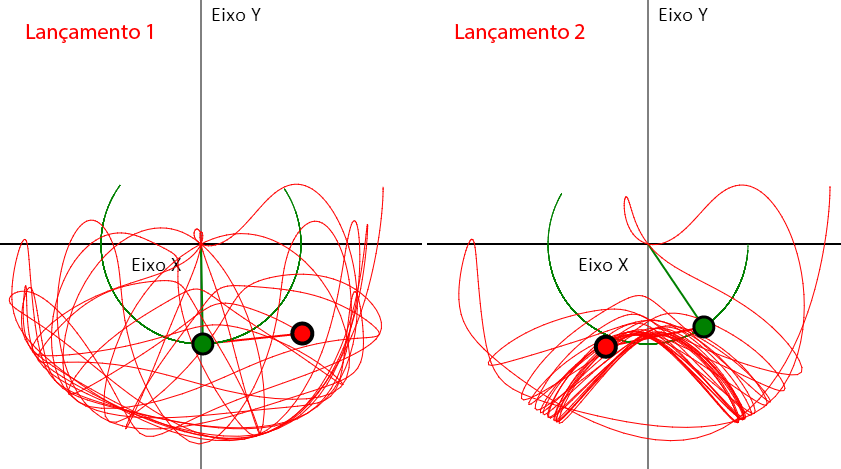
\includegraphics[scale=0.5]{figuras/figura8.png}
\\
\textit{Figura 8: Traços dos pêndulos duplos após $30 s$ de movimento com os parâmetros iniciais definidos.}
\end{center}
\clearpage

\begin{center}
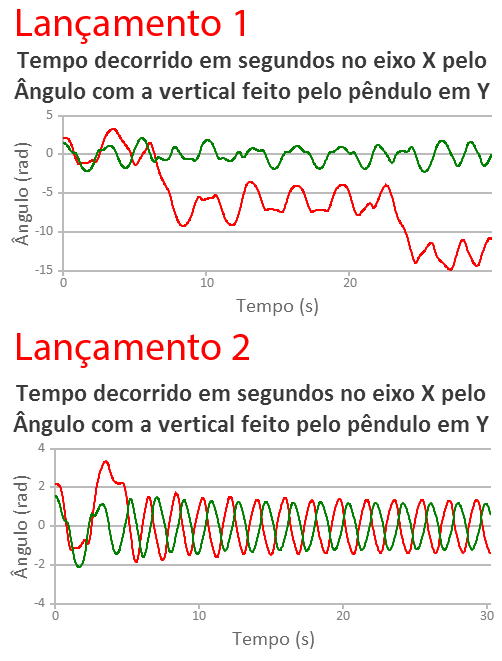
\includegraphics[scale=0.9]{figuras/figura9.png}
\\
\textit{Figura 9: Gráficos dos pêndulos duplos após $30 s$ de movimento com os parâmetros iniciais definidos.}
\end{center}
\clearpage

\begin{center}
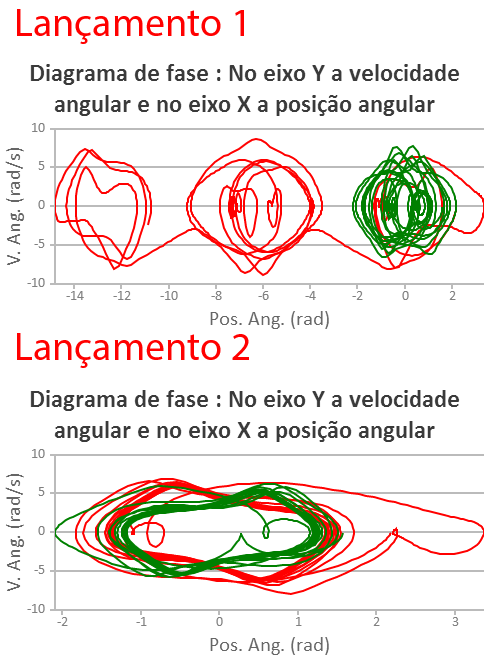
\includegraphics[scale=0.9]{figuras/figura10.png}
\\
\textit{Figura 10: Diagramas de fase dos pêndulos duplos após $30 s$ de movimento com os parâmetros iniciais definidos.}
\end{center}

Através destes gráficos, podemos confirmar o movimento caótico que pode ser causado a partir de mesmos parâmetros iniciais.
\clearpage

\chapter*{Conclusões}
\addcontentsline{toc}{chapter}{Conclusões}
De fato, os 2 tipos de pêndulos apresentados mostram resultados interessantes e que são mais fáceis de analisar do que um modelo real. 

O primeiro, o pêndulo impulsionado, apresenta a mudança de ponto estável conforme variamos os parâmetros de oscilação do pivô. Em outros parâmetros podemos avaliar o movimento caótico que este apresenta.

Já o pêndulo duplo nos dá momentos interessantes de avaliação de como o caos age em sistemas relativamente simples.

Finalmente, estes applets desenvolvidos em HTML5 conseguem ser uma nova ferramenta de estudo e ensino por sua fácil utilização em dispositivos diferentes e por possuir uma melhor facilidade de desenvolvimento.
\clearpage

\chapter*{Apêndice A - Método de Runge-Kutta de 4ª Ordem}
\addcontentsline{toc}{chapter}{Apêndice A - Método de Runge-Kutta de 4ª Ordem}
\section*{Apresentação}
\addcontentsline{toc}{section}{Apresentação}

Em análise numérica, os métodos de Runge-Kutta formam uma importante família de métodos iterativos implícitos e explícitos para resolução numérica de soluções de equações diferenciais ordinárias.

Neste projeto utilizamos o método de 4ª ordem, sendo este o mais utilizado. Existem os métodos de ordem inferiores e superiores, mas para nossos propósitos o de 4ª ordem é o suficiente.

Vamos considerar uma EDO com PVI:
\begin{center}
$
\left \{
\begin{array}{l}
y^{'} = f(t,y) \\
y(t_{0}) = y_{0} \\
\end{array}
\right.
$
\end{center}
Com um passo $h > 0$, devemos calcular:
\begin{center}
$
\begin{array}{l}
k_{n1} = f(t_{n},y_{n}) \\
k_{n2} = f(t_{n} + \dfrac{h}{2} ,y_{n} + \dfrac{h}{2}k_{n1}) \\[3mm]
k_{n3} = f(t_{n} + \dfrac{h}{2} ,y_{n} + \dfrac{h}{2}k_{n2}) \\[3mm]
k_{n4} = f(t_{n} + h,y_{n} + hk_{n3}) \\
\end{array}
$
\end{center}
Para então, obter:
\begin{center}
$
y_{n + 1} = y_{n} + \dfrac{h}{6}\left( k_{n1} + 2k_{n2} + 2k_{n3} + k_{n4} \right)
$
\end{center}
Este é, então, o método mais utilizado em simulações físicas.
\clearpage

\section*{Generalizando para várias variáveis}
\addcontentsline{toc}{section}{Generalizando para várias variáveis}

Conforme visto em nossas deduções, as nossas equações não dependem de somente uma variável e sim várias.

O método de Runge-Kutta pode ser ampliado para estas equações, basta que haja uma transformação de variáveis para obter um sistema de equações diferenciais.

Então, suponha que tenhamos $m$ variáveis com $m$ equações:

\begin{center}
$
\left \{
\begin{array}{c}
x_{1}^{'} = f_{1}\left(x_{1},x_{2},...,x_{m} \right) \\
x_{2}^{'} = f_{2}\left(x_{1},x_{2},...,x_{m} \right) \\
\vdots \\
x_{m}^{'} = f_{m}\left(x_{1},x_{2},...,x_{m} \right) \\
\end{array}
\right.
$
\end{center}
Note que do lado direito não temos derivadas e que do lado esquerdo temos somente derivadas de primeira ordem.Estas equações podem ser resumidas na forma vetorial:
\begin{center}
$
\bar{\textbf{x}}^{'} = \bar{\textbf{f}}\left(\bar{\textbf{x}}\right)
$
\end{center}
onde $\bar{\textbf{x}} = \left(x_{1},x_{2},...,x_{m}\right)$ é o vetor das variáveis e
$ \bar{f} = \left(f_{1},f_{2},...,f_{m}\right) $ o "vetor" das funções.Então, vamos definir
o vetor de variáveis no passo $n$ e $n+1$:
\begin{center}
$
\begin{array}{c}
\bar{\textbf{x}}_{n} = \left(x_{1,n},x_{2,n},...,x_{m,n}\right) \\
\bar{\textbf{x}}_{n + 1} = \left(x_{1,n + 1},x_{2,n + 1},...,x_{m,n + 1}\right) 
\end{array}
$
\end{center}
O método fica, então:
\begin{center}
$
\begin{array}{c}
\bar{\textbf{a}}_{n}  = \bar{f}\left(\bar{\textbf{x}}\right) \\[3mm]
\bar{\textbf{b}}_{n}  = \bar{f}\left(\bar{\textbf{x}} + \dfrac{h}{2}\bar{\textbf{a}}_{n} \right) \\[3mm]
\bar{\textbf{c}}_{n}  = \bar{f}\left(\bar{\textbf{x}} + \dfrac{h}{2}\bar{\textbf{b}}_{n} \right) \\[3mm]
\bar{\textbf{d}}_{n}  = \bar{f}\left(\bar{\textbf{x}} + h\bar{\textbf{c}}_{n} \right)
\end{array}
$
\end{center}
Então, o vetor $ \bar{\textbf{x}}_{n + 1} $ será:
\begin{center}
$
\bar{\textbf{x}}_{n + 1}  = \bar{\textbf{x}}_{n}  + \dfrac{h}{6}\left( \bar{\textbf{a}}_{n} + 2\bar{\textbf{b}}_{n} + 2\bar{\textbf{c}}_{n} + \bar{\textbf{d}}_{n}\right)
$
\end{center}
O vetor $ \bar{\textbf{x}}_{n + 1} $ dará o estado das variáveis após o passo h.

Fica então fácil utilizar qualquer linguagem de programação para programar applets ou mesmo simulações numéricas e obter resultados para inúmeros problemas físicos que não possuem soluções analíticas.
\clearpage


\chapter*{Apêndice B – Frameworks Utilizados}
\addcontentsline{toc}{chapter}{Apêndice B – Frameworks Utilizados}
Nos applets desenvolvidos e utilizados para obter os
resultados foram utilizados alguns frameworks para facilitar o
desenvolvimento.

O primeiro framework foi para organizar o documento HTML,
sendo este o Bootstrap CSS Framework.

Já o utilizado para desenvolvimento em Javascript foram os
seguintes:
\\

1. JQuery  - http://jquery.com

2. Kinetic JS - http://kineticjs.com
\\

Foi utilizado também o framework CanvasJS Charts
(http://canvasjs.com/) para mostrar gráficos das animações em
tempo real.
\\

Não é necessário utilizar estes frameworks para desenvolver
o que foi visto, entretanto a utilização deles facilita muito o
desenvolvimento além de gerar uma organização no código.


\chapter*{Apêndice C – Links para as simulações}
\addcontentsline{toc}{chapter}{Apêndice C – Links para as simulações}
Aqui estão os endereços para os applets que foram apresentados aqui:
\\

Pêndulo Impulsionado:

\href{http://www.ime.unicamp.br/~ra097254/penduloimpulsionado.html}{http://www.ime.unicamp.br/~ra097254/penduloimpulsionado.html}

Pêndulo Duplo:

\href{http://www.ime.unicamp.br/~ra097254/penduloduplo-rk.html}{http://www.ime.unicamp.br/~ra097254/penduloduplo-rk.html}
\\

Basta utilizar um navegador recente (Google Chrome, Mozilla Firefox, Opera , Safari ou Internet Explorer) para que as simulações sejam executadas.Não é necessário instalar nenhum plugin ou software adicional para executá-las.

Caso você tenha problemas na utilização das simulações,verifique se a versão do seu navegador é a mais recente e se todas as configurações relativas a drivers estão corretas em seu computador.
\clearpage


\begin{thebibliography}{9}
\addcontentsline{toc}{chapter}{Bibliografia}

\bibitem{1}
  S. T. Thornton e J. B. Marion,
  Classical Dynamics.
  Thomson Brooks/Cole,
  5a ediçao,
  2004.
  
\bibitem{2}
  W.E Boyce, R.C. DiPrima,
  Equações Diferenciais Elementares e Problemas de Valores de Contorno.
  LTC Books,
  8a ediçao,
  2005.
  
\bibitem{3}
  M.A.G. Ruggiero, V.L.R Lopes,
  Cálculo Numérico - Aspectos Teóricos e Computacionais.
  Pearson Makron Books,
  2a ediçao,
  2006.
 
\bibitem{4}
  Halliday e Resnick,
  Fundamentos da Física, Volume II, Gravitação, Ondas e Calor.
  LTC Books,
  8a ediçao,
  2010.
  
\bibitem{5}
  W3Schools – The world largest web development database, 
  em \href{http://www.w3schools.com/}{http://www.w3schools.com/}.
  
\bibitem{6}
  JQuery - Javascript Framework, 
  em \href{http://www.jquery.com/}{http://www.jquery.com/}.
   
\bibitem{7}
  Kinetic JS – Javascript Framework, 
  em \href{http://kineticjs.com/}{http://kineticjs.com/}.

\bibitem{8}
  CanvasJS Charts – Javascript Charts Framework, 
  em \href{http://canvasjs.com/}{http://canvasjs.com/}.
  
\bibitem{9}
  Bootstrap - CSS Framework, 
  em \href{http://getbootstrap.com}{http://getbootstrap.com}.

\end{thebibliography}

\end{document}